
\chapter{Introducing the comparator}
We first built a relaxation oscillator with different periods, then we tested the LM311 comparator and used it for designing a switch that goes on and off depending on the environment light.

\section{Materials}
\begin{itemize}
\item Comparator LM311
\item Operational amplifier $\mu$A741
\item Phototransistor OP550A
\item Resistors, trimmers, LED, capacitors
\item Power supply RIGOL DP831A
\item Waveform generator RIGOL DG1032
\item Multimeter RIGOL DM3068
\item Oscilloscope RIGOL MS02102A
\end{itemize}
All resistances and capacitances have an error of $5\%$ of the value.

\section{Experimental setup}
\begin{figure}[H]
\centering
\begin{circuitikz}
\draw(0,0) node[op amp] (opamp) {}
%(opamp.+) node[left] {$v_+$}
(opamp.+) ++ (-.3,0) -- (opamp.+) 
(opamp.+) ++ (-.3,0) -- (-1.5,-1.8) to[R,l_=$10\text{k}\Omega$] (1,-1.8) -- (1,0)
(opamp.out) node[right] {$v_o$}
(opamp.down) ++(0,-.5) node[below] {$-v_{cc}$} -- (opamp.down)
(opamp.up) ++ (0,.5) node[above] {$+v_{cc}$} -- (opamp.up);
\draw(-4,.5)node[ground] {}  to[C=$100$nF] (-2,.5) to[short] (opamp.-);
\draw (-1.5,-1.8) to[R,l_=$10\text{k}\Omega$] (-1.5,-3.8)node[ground]{};
\draw(1,0) to[short] (1,2) to[R=$R$] (-2,2) to[short](-2,.5);
\end{circuitikz}
\caption{Relaxation oscillator}
\end{figure}
At first we used the $\mu$A741 (powered with $\pm15$ V) as a comparator in order to build a relaxation oscillator producing a square wave from a capacitor charge and discharge: we chose $R_1 = R_2 = 10.0 \pm 0.5 k\Omega$ and a $100 \pm 5 pF$ capacitor. The circuit has been tested with 5 different values of R in order to have different periods. A measure has been taken also setting the oscilloscope in single mode and then switching on the power supply.\\
We then tested the LM311 both as non-inverting and inverting comparator using $R_L = 1000 \pm 50 \Omega$.\\
Regarding the Schmitt's trigger, we added to the previous circuit the resisteors $R_1 = 10.0 \pm 0.5 k\Omega$ and $R_2 = 100 \pm 5 \Omega$ and analyzed the behaviour at the point when $v_{in}\approx v_{ref}$.\\
\begin{figure}[H]
\centering
\begin{minipage}{.5\textwidth}
\centering
\begin{circuitikz}
\draw(0,0) node[op amp,yscale=-1] (opamp) {}
(opamp.+) node[left] {$v_+$}
(opamp.-) node[left] {$v_-$}
%(opamp.+) ++ (-.3,0) -- (opamp.+) 
(opamp.out) node[right] {$v_o$}
%(opamp.down) ++(0,-.5) node[below] {$-v_{cc}$} -- (opamp.down)
(opamp.down) to[short] (-.0825,1) node[above] {$+v_{cc}$} 
(opamp.up) to[short] (-.0825,-1) node[below] {$-v_{cc}$};
\draw(1.1,2)node[above]{$v_{cc}$}to[R=$R_L$,o-](1.1,0); 
\draw(opamp.up) ++ (.6,.36)node[right,yshift=-.3em]{\scriptsize$1$} to[short](.515,-.35)node[ground]{};
\draw(0,0)node[xshift=-.3em]{LM311};
\end{circuitikz}
\end{minipage}%
\begin{minipage}{.5\textwidth}
\centering
\begin{circuitikz}
\draw(0,0) node[op amp,yscale=-1] (opamp) {}
(opamp.+) node[left] {$v_+$}
%(opamp.-) node[left] {$v_-$}
(opamp.-) ++ (-.3,0) -- (opamp.-) 
(opamp.out) node[right] {$v_o$}
%(opamp.down) ++(0,-.5) node[below] {$-v_{cc}$} -- (opamp.down)
(opamp.down) to[short] (-.0825,1) node[above] {$+v_{cc}$} 
(opamp.up) to[short] (-.0825,-1) node[below] {$-v_{cc}$};
\draw(1.1,2)node[above]{$v_{cc}$}to[R=$R_L$,o-](1.1,0); 
\draw(opamp.up) ++ (.6,.36)node[right,yshift=-.3em]{\scriptsize$1$} to[short](.515,-.35)node[ground]{};
\draw(0,0)node[xshift=-.3em]{LM311};
\draw(opamp.-) ++ (-.3,0) -- (-1.5,-1.8) to[R,l_=$10\text{k}\Omega$] (1,-1.8) -- (1,0)
(-1.5,-1.8) to[R,l_=$100\Omega$] (-1.5,-3.8)node[ground]{};
\end{circuitikz}
\end{minipage}
\caption{Comparator test with and without Schmitt's trigger}
\end{figure}
At last, we built the twilight switch with circuit \ref{interruttorecrepuscolare}. We used a phototransistor (which gives us a current which intensity is based on the light one) followed by an op-amp stage (for converting the current in voltage): due to the fact that che current from the phototransistor is very small we had to adjust carefully the op-amp offset in order to avoid sistematic errors. In the last stage we used the LM311 comparator to switch a led on and off comparing a reference voltage $v_{ref}$ with the op-amp stage output.
\begin{figure}[H]
\centering
\begin{circuitikz}
%\draw[help lines] (-5,-2) grid (5,3);

%STAGE PHOTO TRANSISTOR
\draw(-5,1)node[above]{$-v_{cc}$}to[R,o-](-5,-1)node[ground]{};
\draw(-3.3,.865)node[npn,photo](npn){};
\draw[-stealth](npn.E) -- (-4.71,.09);

%STAGE CONVERTER
\draw(npn.C)to[short](-2.7,1.635);
\draw(-1.52,1.1462) node[op amp] (opamp1) {};
\draw(opamp1.+)to[R,l_=$1\text{k}\Omega$](-2.7,-1)node[ground]{};
\draw(-1.52,1.1462)node[xshift=-.3em]{$\mu$A741};
\draw(opamp1.-)to[short](-2.7,3.2)to[R=$1\text{M}\Omega$](-.3335,3.2)to[short](opamp1.out)
(opamp1.up)--++(0,.5)node[above]{$+v_{cc}$}
(opamp1.down)--++(0,-.5)node[below]{$-v_{cc}$};


%STAGE COMPARATOR
\draw(2.359,.655) node[op amp,yscale=-1] (opamp) {}
(opamp.down) to[short] (2.2765,1.655) node[above] {$+v_{cc}$}
(opamp.up) to[short] (2.2765,-0.345) node[below] {$-v_{cc}$};
\draw(opamp.up) ++ (.6,.36)node[right,yshift=-.3em]{\scriptsize$1$} to[short](2.874,0.305)node[ground]{};
\draw(2.359,.655)node[xshift=-.3em]{LM311};
\draw(opamp.-)to[R=$100\Omega$,-o](-.5,0.155)node[left]{$v_{ref}$};
\draw(opamp1.out)to[R=$100\Omega$](opamp.+);
\draw(opamp.+)to[short](1.17,2.5)to[R=$10\text{k}\Omega$](3.5,2.5)to[short](3.5,.655);
\draw(opamp.out)to[short](4.5,.655);
\draw(4.5,3.7)node[above]{$+v_{cc}$}to[R=$R_L$,o-](4.5,1.9)to[leDo](4.5,.655);
\end{circuitikz}
\caption{Twilight switch}\label{interruttorecrepuscolare}
\end{figure}

\section{Data Analysis}
\begin{figure}[H]
\centering
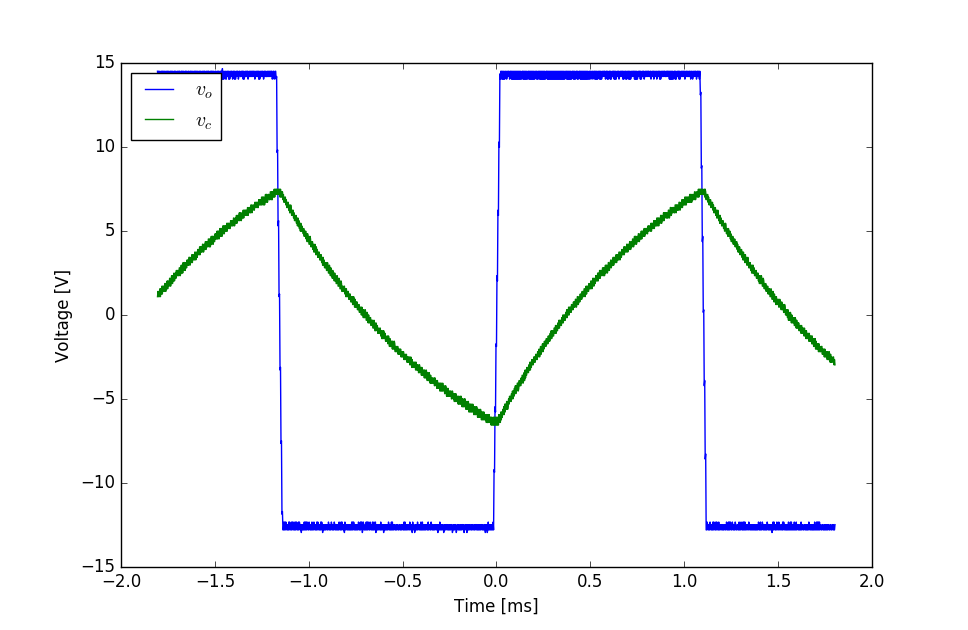
\includegraphics[width=.7\textwidth]{5/10k_plot.png}
\caption{op-amp output $v_o$ and capacitor voltage $v_c$ with $R=10\text{k}\Omega$}
\end{figure}
The oscillator period is related to the resistor $R$ as follows:
\[T = 2RC\ln \left(1+\frac{2R_1}{R_2}\right)\]
where $C$ is the capacitor and $R_1=R_2=10\text{k}\Omega$. Using the values measured with the multimeter we plotted a theoretical curve in funciton of $R$ and we can see that the data are on that line: in fact the slope measured thanks to a linear fit $218.12 \pm 0.06 F$ is in perfect accordance with the expected value $220 \pm 3 F$ (but we have to say that only five points don't represent a great pool on which to do a linear regression and statistics). The errors needed for the regression have been provided by the oscilloscope and multimeter resolution. 
\begin{figure}[H]
\centering
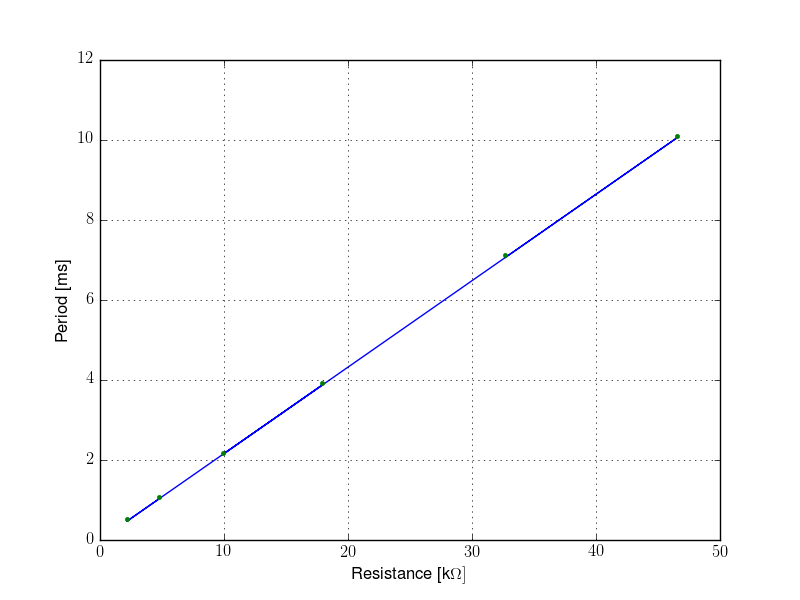
\includegraphics[width=.7\textwidth]{5/fit.png}
\caption{Data (green dots) and theoretical curve (blue line)}
\end{figure}
We then checked our comparator behaviour: actually it gave an high output when the voltage at the non invertent pin was higher than the other input and a low one when it became lower. The opposit effect happened with the inverting configuration.
In the following figures we can see the difference in the comparator output with and without the Schmitt's trigger: when the Schmitt's trigger wasn't present, the noise caused an unwanted on-off repeated toggle. The Schmitt's trigger raises and lowers time to time the threshold of the switching in order to avoid this problem.
\begin{figure}[H]
\begin{minipage}{.5\textwidth}
\centering
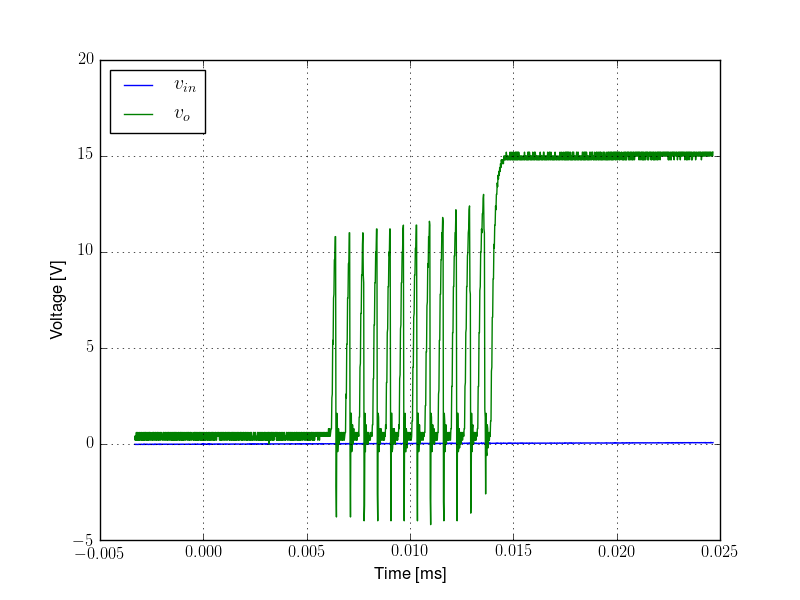
\includegraphics[width=\textwidth]{5/noise.png}
\caption{Without Schmitt's trigger}
\end{minipage}%
\begin{minipage}{.5\textwidth}
\centering
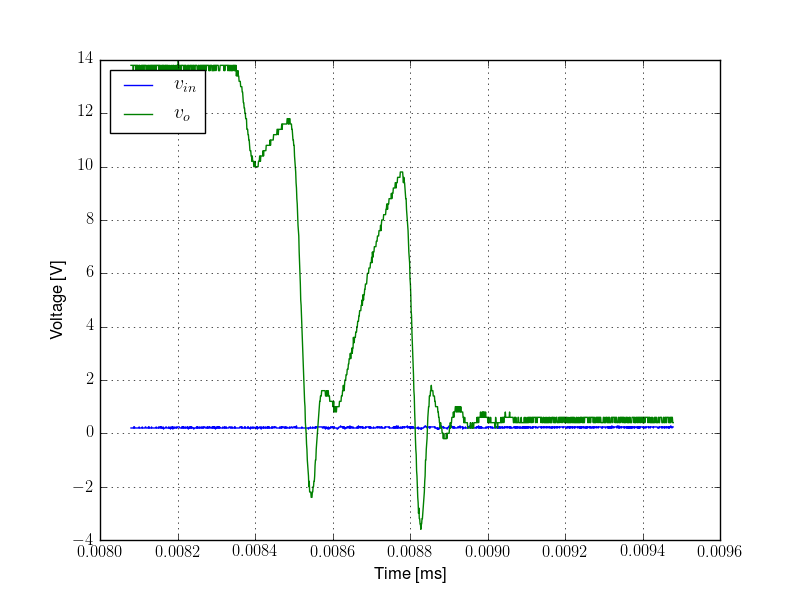
\includegraphics[width=\textwidth]{5/schmitt.png}
\caption{With Schmitt's trigger}
\end{minipage}
\end{figure}
Lastly, the circuit based on the phototransistor: once mounted, we verified its correct functioning noticing that when the light was weaker than a fixed amount it actually switched on the LED and kept it lighted till a new sufficent brightness increase.\\
We were also able to choose the threshold for the switching by adjusting the voltage reference $v_{ref}$ using a trimmer.\\
Below a photo of this circuit. 
\begin{figure}[H]
\centering
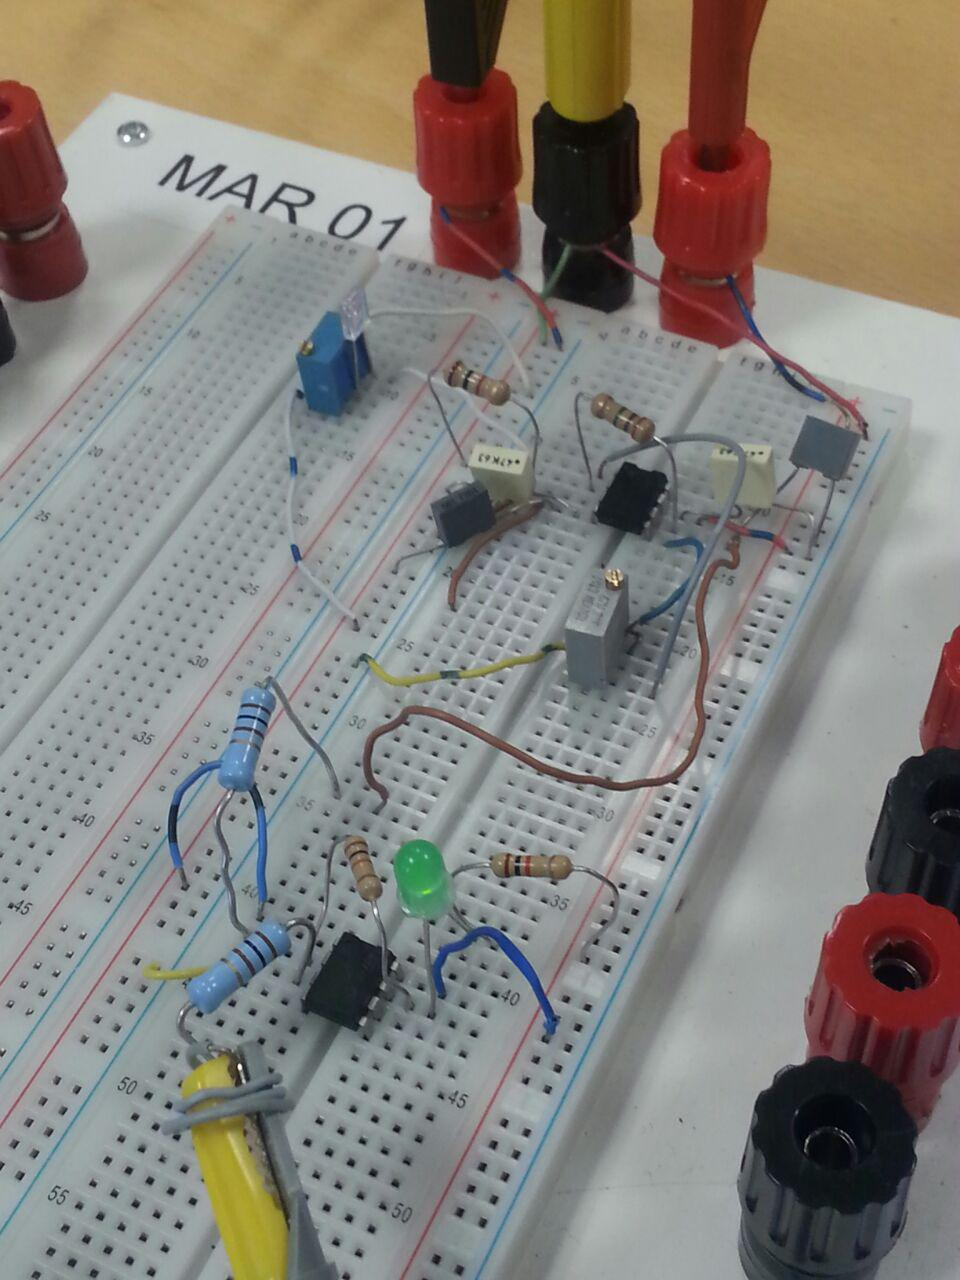
\includegraphics[width=.6\textwidth]{5/sw.jpg}
\caption{Twilight switch circuit}
\end{figure}
